\title{Memoria de seguimiento}
\author{
        Beñat Agirre Arruabarrena \\
        b.agirre@alumnos.upm.es \\
}
\date{\today}

\documentclass[11pt]{article}
\usepackage[spanish]{babel}
\usepackage{graphicx}
\graphicspath{ {./images/} }
\usepackage{pdfpages}
\usepackage{fullpage}

\begin{document}
\maketitle
\tableofcontents
\newpage

%%%%%%%%%%%%%%%%%%%%%%%%%%%%%%%%%%%%%%%%%%%%%%%%%%%%%%%%%%%%%%%%%%%%%%%%%%%%%%%%%%%%%%%%%%%%%%%%%%%%%%%%
\section{Resumen del trabajo realizado}
\begin{enumerate}
    \item Analizar el funcionamiento de las herramientas de Linked Data Geográfico utilizadas por el Grupo de
        Ingeniería Ontológica y determinar si existen nuevas alternativas mejores.

    \item Preparar el nuevo entorno de desarrollo con el SDK de PDI 9 y crear el fichero pom.xml de maven para
        gestión automática de dependencias de tripleGeoKettle.

    \item Comenzar a portar tripleGeoKettle y la toolchain de transformaciones desde GEOKettle a PDI 9.

    \item Escribir primeros apartados de la memoria
\end{enumerate}


%%%%%%%%%%%%%%%%%%%%%%%%%%%%%%%%%%%%%%%%%%%%%%%%%%%%%%%%%%%%%%%%%%%%%%%%%%%%%%%%%%%%%%%%%%%%%%%%%%%%%%%%
\section{Explicación y justificación de las modificaciones al Plan de Trabajo}

Desde que se publicó ``A sustainable process and toolbox for geographical linked data generation and
publication: a case study with BTN100'' en 2019, GeoKettle ha dejado de estar soportado. La pagina oficial y de
documentación ya no están disponibles.
Un objetivo de este TFG era dar soporte GeoPackage a GeoKettle. No tiene sentido desarrollar soluciones de
``modernización'' sobre software abandonado. Por tanto, se ha optado por actualizar la herramienta.

Algunas funcionalidades de GeoKettle se integraron en PDI directamente y otras desaparecieron.
Actualmente, el soporte GIS de Pentaho está dentro de PDI Spoon y además hay algunas funcionalidades más en
 el plugin llamado pentaho-gis-plugins. Se actualizará la fase de añadir soporte GeoPackage a GEOKettle a:
``replicar la funcionalidad y las transformaciones de GeoKettle y TripleGeo en la suite PDI.'' Si es sencillo,
se considerará también dar soporte a GeoPackage.

\subsection{Revisión de la lista de objetivos del trabajo}
\begin{itemize}
    \item Replicar la funcionalidad y las transformaciones de GeoKettle y TripleGeo en la suite PDI
    \item Dar soporte GeoPackage a la herramienta GeoKettle y su plugin para transformar a RDF
    \item Realizar un procesado completo de todos los datos del IGN para generar este tipo de formato.
\end{itemize}

\subsection{Revisión de la lista de tareas}
La lista de tareas no ha cambiado ya que era bastante general.
\begin{itemize}
    \item Análisis del formato GeoPackage y herramientas asociadas: 20\%
    \item Diseño de soluciones: 20\%
    \item Implementación de soluciones: 40\%
    \item Evaluación: 10\%
    \item Documentación: 10\%
\end{itemize}

\subsection{Revisión del Diagrama de Gantt}
El diagrama de Gantt tampoco cambia porque no ha cambiado la lista de tareas.
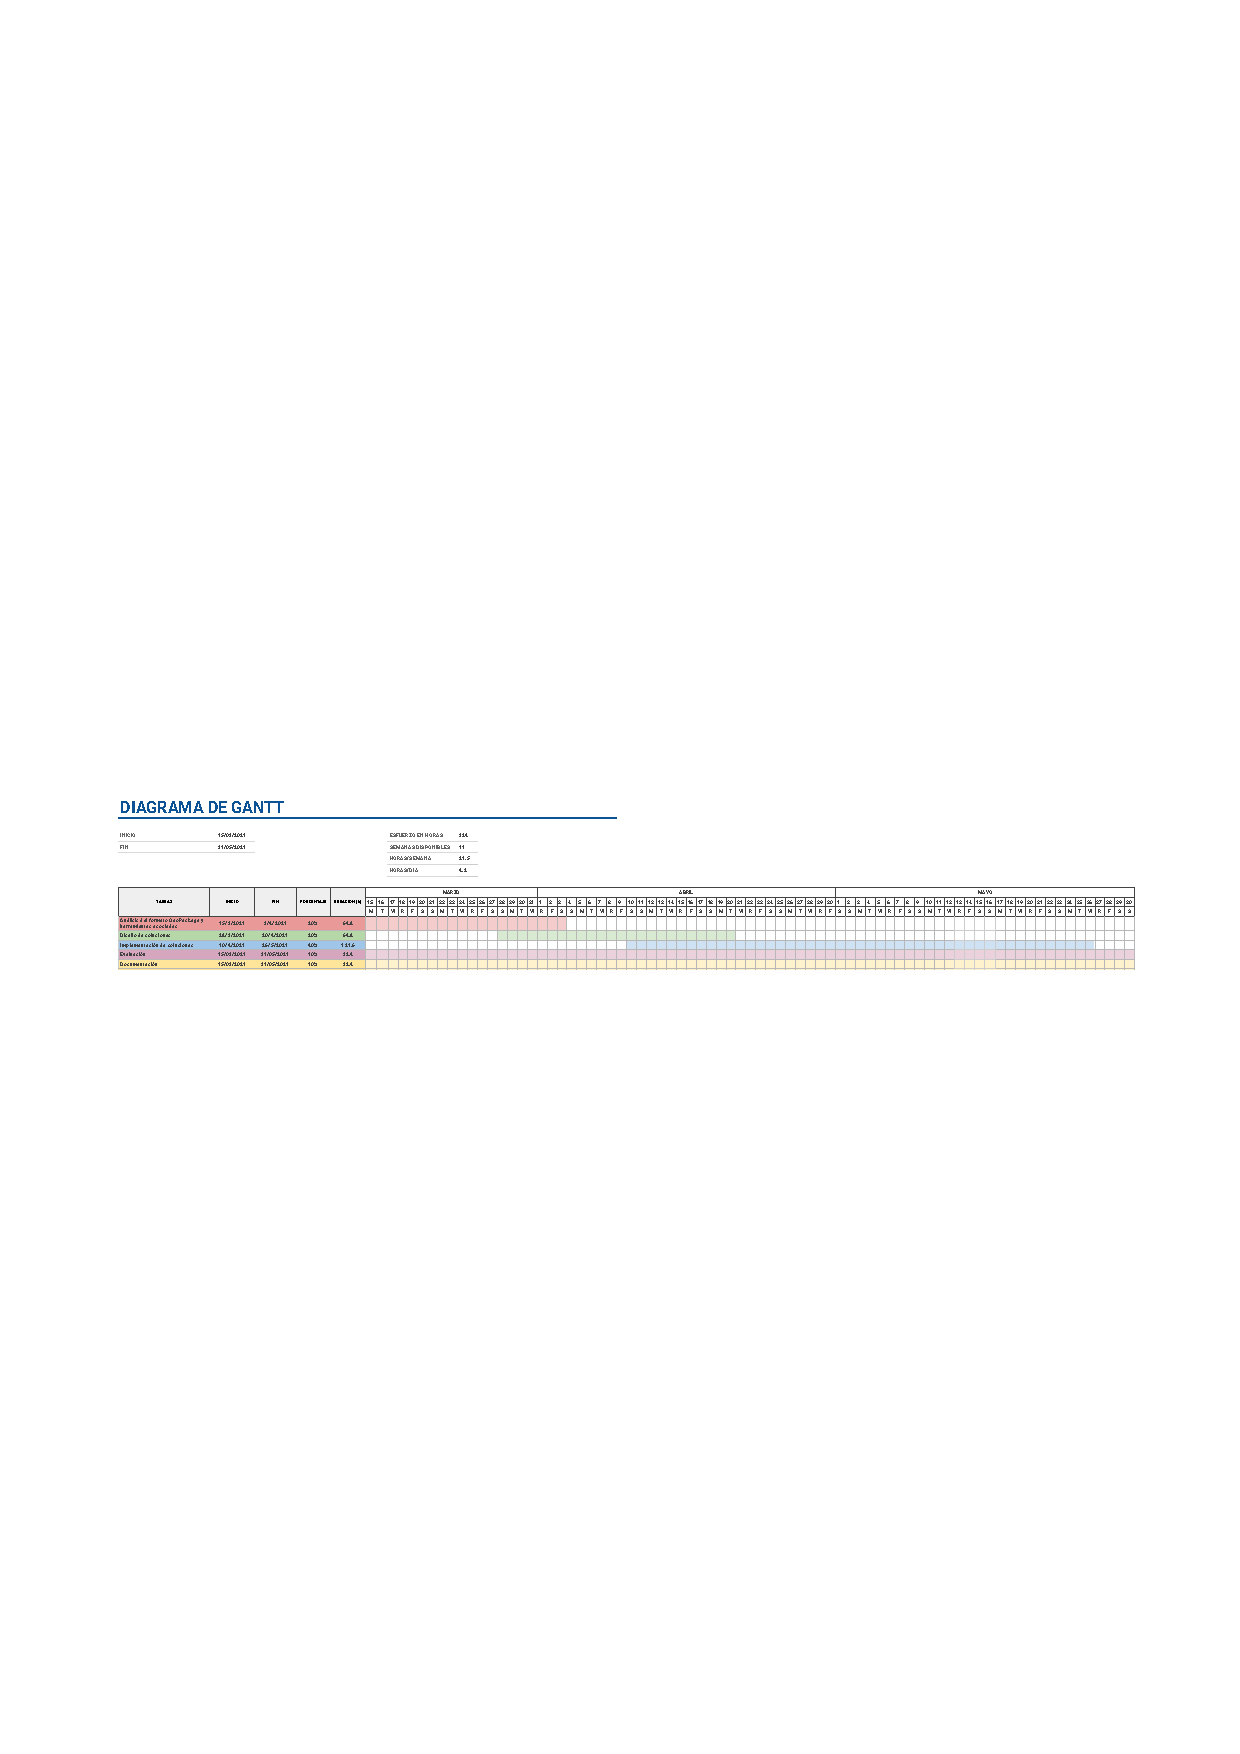
\includepdf[pages=-]{../plan_de_trabajo/Gantt.pdf}

\section{Borrador de la Memoria Final}
A continuación se adjunta el borrador completo de la memoria final:

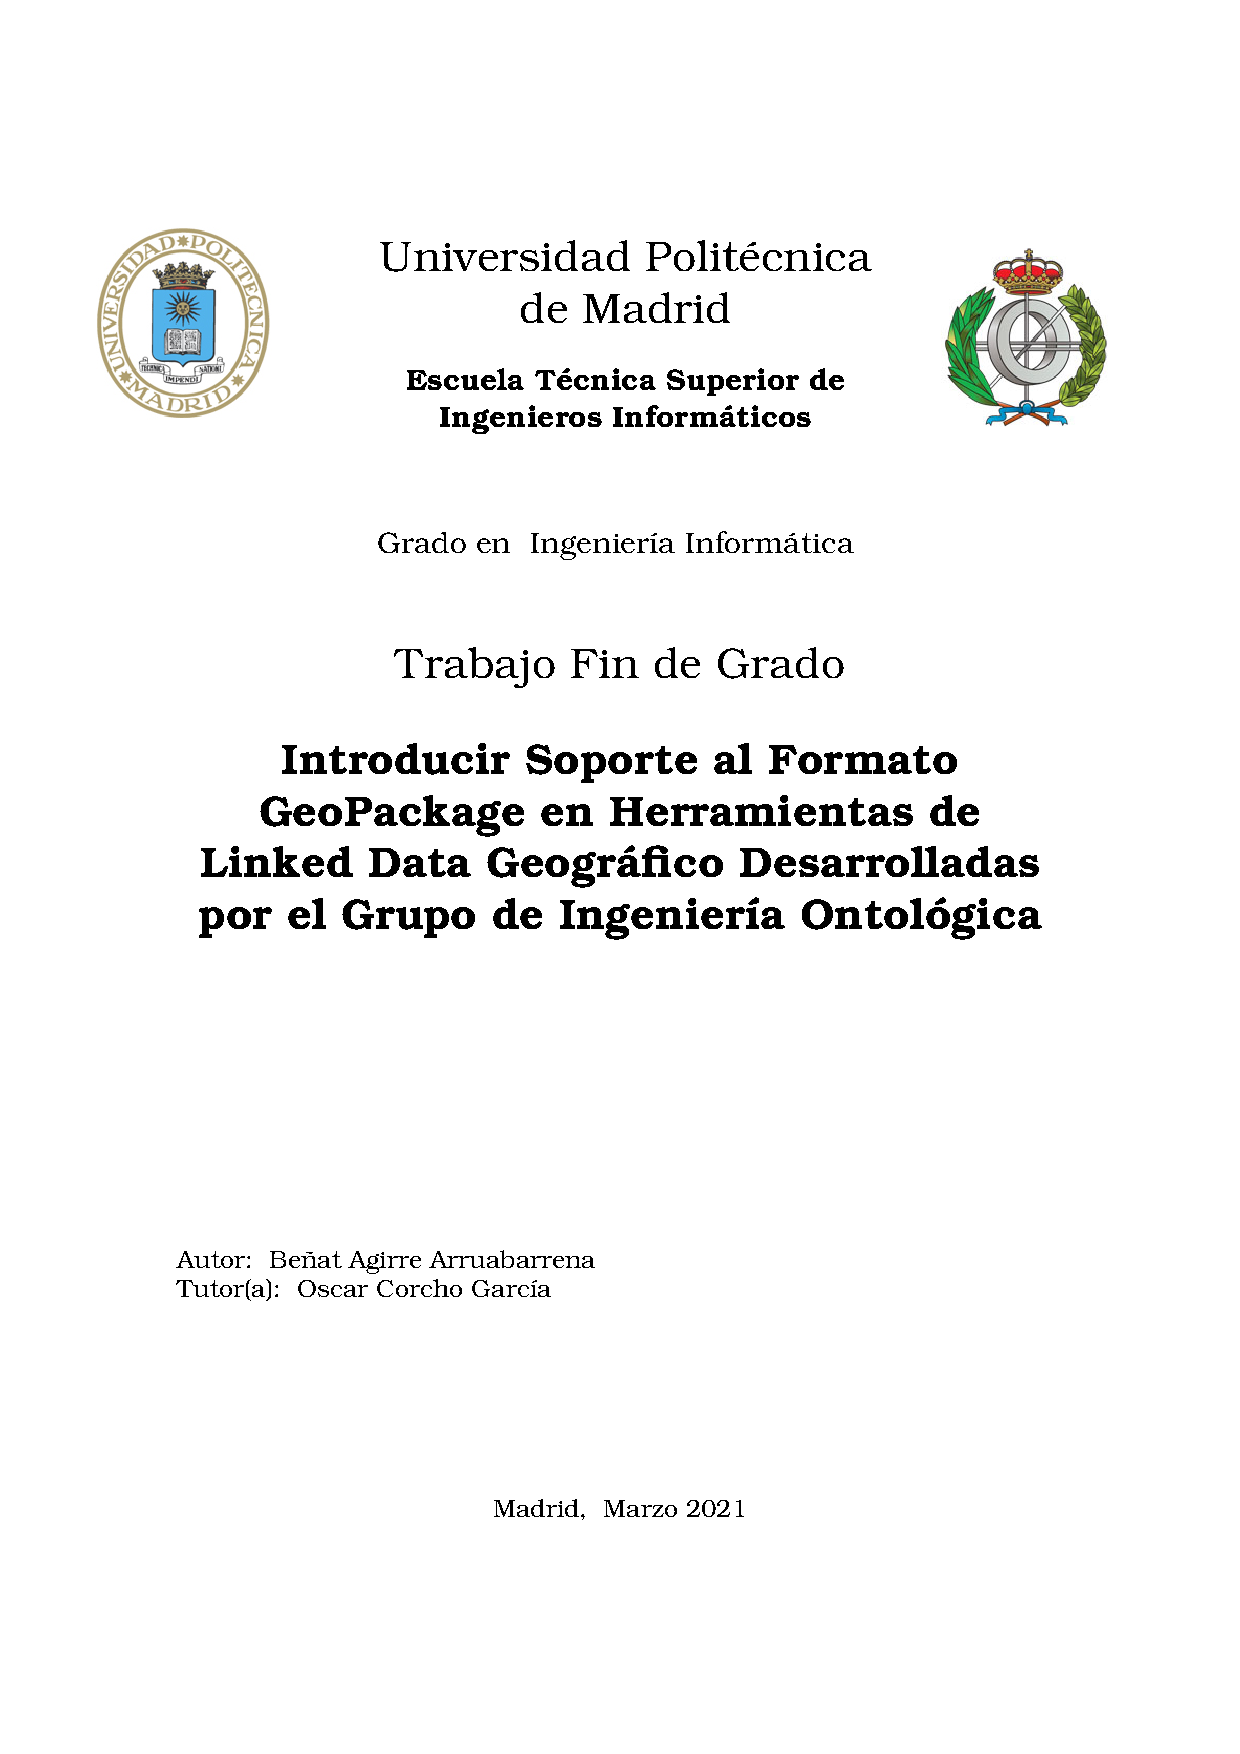
\includepdf[pages=-]{../memoria/plantilla_TFG.pdf}
\end{document}
